\chapter{Data Exploration and Scheduling Problem Building Blocks}
\label{chapter: Problem Definition}

%%%%%%%%%%%%%%%%%%%%%%%%%%%%%%%%%%%%%%%%%%%%%%%%%%%%%%%%%%%%%%%%%%%%%%%%%%%%%%% SECTION %%%%%%%%%%%%%%%%%%%%%%%%%%%%%%%%%%%%%%%%%%%%%%%%%%%%%%%%%%%%%%%%%%%%%%%%%%%%%%

In this chapter we re-introduce the problem assigned to us by Royal Mail in a greater level of detail. Sections \ref{section: problem outline}-\ref{section: Input Parameters} walk the reader through a more detailed description of the problem to introduce them to the main elements that constitute the problem as well as give them an idea of Royal Mail's current practices through a series of examples. They also outline the motivation behind solving this problem, and provide arguments justifying why this is a problem worthwhile solving, with great potential for efficiency gains despite the complexity involved in obtaining a solution. 

\vspace{\baselineskip}
\noindent
Following the description of the problem, Section \ref{section: Data Exploration} continues by outlining the structure of the historical data supplied by Royal Mail, and the steps taken to bring the dataset in the form that was utilised in the modelling portion of the project. The \textbf{finalised} form of the dataset described at the end of the Data Cleaning section \ref{section: Data Cleaning} constitutes the foundation upon which this dissertation will derive feasible, and efficient schedules. The chapter concludes with Sections \ref{section: Redefined Dataset}-\ref{fig: Wave-instances.} describing the processes behind the generation of two unique instances of the problem that will be utilised to conduct more targeted experiments in Chapter \ref{chapter: 2-Evaluating Royal Mail Historical Data}. 

\vspace{\baselineskip}
\noindent
All in all, this chapter gives a more detailed overview of the problem, as well as a detailed description of the dataset provided by our Industrial Liaison, and the steps taken to prepare it for use in our experiments. 

%%%%%%%%%%%%%%%%%%%%%%%%%%%%%%%%%%%%%%%%%%%%%%%%%%%%%%%%%%%%%%%%%%%%%% Section %%%%%%%%%%%%%%%%%%%%%%%%%%%%%%%%%%%%%%%%%%%%%%%

\section{General Context}
\label{section: problem outline}
Each of Royal Mail's \textbf{Mail Centres (MC)} upon receiving the mail collected from each \textbf{Delivery Office (DO)} will sort it and then decide which portions of it need to be redistributed to DOs belonging to the same MC the following day. Our goal is to structure the delivery itinerary for each MC, for the portion of the post that will remain within the circulation of that MC. 


\vspace{\baselineskip}
\noindent
The day before a piece of mail is delivered, the MC responsible for it will have a set of round-trips that need to be completed. At its disposal, each MC has a crew of \textbf{HGV drivers}, that will complete those trips. Our objective, is to schedule those trips in a more efficient manner than Royal Mail's current scheduling practices, that minimises the time that drivers spend performing \textbf{non-essential} activities that could be performed by lower-grade employees. The process of creating those schedules can be resolved into two sub-components. \textbf{Firstly}, decide which trips are completed by each driver. \textbf{Secondly}, decide how to sequence the trips assigned to each driver. In allocating trips to a driver we need to respect some restrictions imposed by certain parameters on whether a trip can be allocated to each specific driver, on a particular instant in time. These restrictions are driven by the EU regulations\footnote{Further explained in Appendix \ref{section: EU rules}} around HGV drivers, in particular the \textit{driving} and \textit{working} time directives. However, for the purposes of this dissertation we neglect those, hence our focus is solely concerned with the task of finding the \textbf{room} available \textbf{for optimisation}. Following that, it should be straightforward to make the modelling more realistic by introducing those important constraints that ensure the utmost legality of the schedules and it is one of the direction considered for future work\footnote{Further explained in Section \ref{section: Addition of the Meal Relief Constraint} of Chapter \ref{chapter: Future Directions}} on the problem. 

\vspace{\baselineskip}
\noindent
As mentioned in the Introduction chapter of the report, we only focus on the \textbf{scheduling} aspect of the problem, and consider the routes to be fixed, hence we do not focus on the \textit{Vehicle Routing} point of view.


%%%%%%%%%%%%%%%%%%%%%%%%%%%%%%%%%%%%%%%%%%%%%%%%%%%%%%%%%%%%%%%%%%%%%% Figure %%%%%%%%%%%%%%%%%%%%%%%%%%%%%%%%%%%%%%%%%%%%%%%

\begin{figure}
    \centering
	\begin{tikzpicture}[node distance=2cm,>=stealth',bend angle=45,auto,rotate=90,transform shape]%picture #1

      \tikzstyle{place}=[circle,thick,draw=black!75,fill=white!20,minimum size=10mm]
      \tikzstyle{red place}=[place,draw=red!75,fill=red!20]
      \tikzstyle{transition}=[rectangle,thick,draw=black!75,
      			  fill=black!20,minimum size=10mm]
    
      \tikzstyle{every label}=[black]
    
      \begin{scope}
        
        
        %All but clients
        \node [place,label={[rotate=-90]center:DO}] (w1)                                    {};
        \node [place, draw=white,label={[rotate=-90]center:Trip A}] (c1) [below of=w1]                      {};
        \node [place, line width=0.8mm,label={[rotate=-90]center:MC}] (s)  [below of=c1] {};
        \node [place, draw=white,label={[rotate=-90]center:Trip B}] (c2) [below of=s]                       {};
        \node [place,label={[rotate=-90]center:DO}] (w2) [right of=c2]                      {}
            edge [pre,bend right]                (s);
    
        %boxes w/ Clients
        \node [transition,label={[rotate=-90]center:Client}] (e1) [left of=c1] {}
          edge [pre,bend left]                  (w1)
          edge [post,bend right]                (s);
    
        \node [transition,label={[rotate=-90]center:Client}] (e2) [left of=c2] {}
          edge [post,bend left]                 (s);
    
        \node [transition,label={[rotate=-90]center:Client}] (l1) [right of=c1] {}
          edge [pre,bend left]                  (s)
          edge [post,bend right] node[swap] {} (w1);
    
        \node [transition,label={[rotate=-90]center:Client}] (l2) [below of=c2] {}
          edge [pre,bend right]                 (w2)
          edge [post,bend left]  node {}       (e2);
      \end{scope}

\end{tikzpicture}%picture #1
    \qquad
    %picture #-5

    \caption{An example of a typical duty consisting of two \textbf{round-trips} (i.e. atomic blocks), both starting and concluding at the MC.}
    \label{fig:Atomic block}%
\end{figure}

\vspace{\baselineskip}
\noindent
At the start of every working day, a driver is assigned their day's itinerary. The dataset provided to us, contains such historical itineraries for every driver per each day of the week. The task at hand, is to use those historical itineraries to \textbf{propose optimised schedules for each day}, which will \textbf{be optimal in their use of the drivers' time.}

%%%%%%%%%%%%%%%%%%%%%%%%%%%%%%%%%%%%%%%%%%%%%%%%%%%%%%%%%%%%%%%%%%%%%% Section %%%%%%%%%%%%%%%%%%%%%%%%%%%%%%%%%%%%%%%%%%%%%%%

\section{Building Blocks}
\label{section: Input Parameters}
The optimised schedules will be based on historical schedules supplied in the form of a dataset\footnote{Further explained in Section \ref{section: Data Exploration}} by Royal Mail. The context of the problem involves historical schedules for a \textbf{model week} for the Exeter MC. The \textit{definition} of a \textbf{schedule} is the collection of duties that are assigned to drivers for each day of the week. Each driver is assigned their \textbf{duty} (or else their shift) for the day which constitutes their itinerary for that day. Their duty instructs them to fulfill a number of round-trips each day. Their first trip of the day commences from the Exeter MC, and following a number of visits to external locations their final trip concludes at the Exeter MC, at the end of their day's itinerary. The duties are composed of one or more units of the following two key data points featured throughout the dataset:

%%%%%%%%%%%%%%%%%%%%%%%%%%%%%%%%%%%%%%%%%%%%%%%%%%%%%%%%%%%%%%%%%%%%%% Bullet Points %%%%%%%%%%%%%%%%%%%%%%%%%%%%%%%%%%%%%%%%%%%%%%%

\begin{itemize}
    \item \underline{\textbf{Activity}}: The main \textit{unit of information} signifying the completion of a task.  Each activity has a \texttt{processing\_time} associated with it, informing us of how long the job that it contains takes to be completed. The jobs contained in an activity could be loading/unloading of the mail, driving time between two locations etc\footnote{A comprehensive list of all the instances of activities is cited in Table \ref{table:Activity List} of Appendix \ref{section: Appendix Activities Feaure in the Dataset}.}.
    
    \item \underline{\textbf{Atomic Interval (block)}}: The building blocks that make up a \textbf{duty}. A block represents a \textbf{single round-trip} that commences at the MC and through completing stops at various external locations, concludes again at the MC, see Figure \ref{fig:Atomic block}. Those locations are either Royal Mail's or clients' premises. Mathematically it is defined as a \textit{block of time}, during which a collection of \textbf{activities} take place. Multiple such atomic intervals are often featured inside a single duty. The intervals are completely \textit{tightly packed} in the sense that activities are rigidly in place, with no idle time going to waste in between two adjacent activities inside a block. The intervals are characterised as \textit{atomic}, to highlight their firm structure that cannot be broken into sub-components i.e. smaller sets of activities. To move a block, one cannot simply move a portion of it but has to move it in its entirety. 
\end{itemize}

%%%%%%%%%%%%%%%%%%%%%%%%%%%%%%%%%%%%%%%%%%%%%%%%%%%%%%%%%%%%%%%%%%%%%% Figure %%%%%%%%%%%%%%%%%%%%%%%%%%%%%%%%%%%%%%%%%%%%%%%

%Two images in one, illustrating atomic block
\begin{figure}%
    \centering
    \subfloat[The set relationship between the various Input Parameters of our problem.]{
    \begin{tikzpicture}[scale=0.6, every node/.style={scale=0.9}]
    \node[set,fill=blue4,text width=6.5cm,label={[below=148pt of rea,text opacity=1]\textit{Schedule}}] 
        (nat) at (0,-0.7)  (rea) {};
    \node[set,fill=blue3,text width=5cm,label={[below=108pt of rea,text opacity=1]\textit{Duties}}] 
      (nat) at (0,-0.5)  (rea) {};
    \node[set,fill=blue2,text width=3.5cm,label={[below=66pt of int]\textit{Atomic Blocks}}] 
      (int) at (0,-0.3)  {};
    \node[set,fill=blue1,text width=2cm] (nat) at (0,0) {\textit{Activities}};
    \end{tikzpicture}}%picture #1
    \qquad
    %picture #2
    \subfloat[Structure of a Duty, showing $Activities$ ($A_{i}$) inside $Atomic \; Blocks$ which themselves are inside a $Duty$.]{\raisebox{5em}{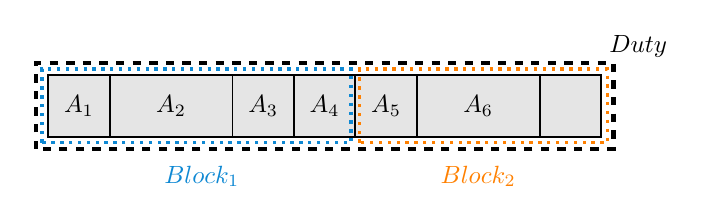
\begin{tikzpicture}[line width=.7pt,scale=0.78, every node/.style={scale=0.9}]
        %Activities
        \draw[fill=gray!20] (0,0)node[below]{} rectangle(1,1);
        %%%%%%%%%%%%%%%%%%%%%%%%%%%%%% NOTATION %%%%%%%%%%%%%%%%%%%
        %%%%%%%%%%%%%%%%%%%%%(bottomleft)             (topright)
        \draw[fill=gray!20] (1,0)node[below]{} rectangle(3,1);
        \draw[fill=gray!20] (3,0)node[below]{}rectangle(4,1);
        \draw[fill=gray!20] (4,0)node[below]{}rectangle (5,1)(2.5,1)node[below,yshift=-1.15cm, text=cyan!70!blue]{$\boldsymbol{Block_1}$};
        \draw[fill=gray!20] (5,0)node[below]{}rectangle (6,1);
        \draw[fill=gray!20] (6,0)node[below]{}rectangle (8,1);
        \draw[fill=gray!20] (8,0)node[below]{}rectangle (9,1)(7,1)node[below,yshift=-1.15cm, text=orange]{$\boldsymbol{Block_2}$}(9.605,0.75)node[below,yshift=0.9cm]{$\boldsymbol{Duty}$};
        %Blocks
        %\draw[fill=none, double=gray!40,double distance =1pt] (-0.1,-0.1)node[below]{} rectangle(4.93,1.1);
        %\draw[fill=none, double=red,double distance =1pt] (5.07,-0.1)node[below]{} rectangle(9.1,1.1);
        \draw[fill=none,very thick,dotted,draw=cyan!70!blue] (-0.1,-0.1)node[below]{} rectangle(4.93,1.1);
        \draw[fill=none,very thick,dotted,draw=orange] (5.07,-0.1)node[below]{} rectangle(9.1,1.1);
        %Duty
        \draw[fill=none,ultra thick,dashed] (-0.2,-0.2)node[below]{} rectangle(9.2,1.2);
        
        \path (0.5,.5)node{$A_1$} (2,.5)node{$A_2$} (3.5,.5)node{$A_3$} (4.5,.5)node{$A_4$} (5.5,.5)node{$A_5$} (7,.5)node{$A_6$} (8.5,.5)node{$\dotsi$};
        %%%%%%%(width of label, height)
        \end{tikzpicture}}}
    %end of picture #2
    \caption{Illustrations explaining the nature of the Input Parameters of the problem.}%
    \label{fig:Useful Time}%
\end{figure}

\vspace{\baselineskip}
\noindent
We now focus on two simplified examples that are meant to give the reader a more practical overview of the problem in question. We start off with a dreamt-up example that serves as an illustration that hopefully highlights the foundations of the problem, then transitioning to a more reality-based example that is meant to resemble what typically occurs in a Royal Mail MC.


%%%%%%%%%%%%%%%%%%%%%%%%%%%%%%%%%%%%%%%%%%%%%%%%%%%%%%%%%%%%%%%%%%%%%% Figure %%%%%%%%%%%%%%%%%%%%%%%%%%%%%%%%%%%%%%%%%%%%%%%

\begin{figure}[htb!]
\begin{tikzpicture}
\begin{axis}[
  font=\scriptsize,
  ytick style={draw=none},
  xtick style={draw=none},
  %unit vector ratio*=1 1 1,%1 0.6 1,
  axis lines = middle,
  enlarge x limits = {value=.01,upper},
  enlarge y limits = {value=.05,upper},
  ylabel={\textbf{Duties}},
  xlabel={\textbf{Time (HH:mm)}},
  ylabel near ticks,
  xlabel near ticks,
  const plot,
  stack plots=false,
  area style,
  width=\linewidth,
  height=5cm, %control the height of chart
  %width=\linewidth,height=\textheight,
  ytick={1,...,60},
  yticklabels={},  
  xtick={1,3,...,24},
  %xticklabels = {4,6,8},
  extra y ticks={1,2,3,4},
  extra y tick style={yticklabel={$D_{\pgfmathprintnumber{\tick}}$}}
  ] 
  
  const char *colour[12] = { "yellow", "orange", "red!20", "gray", "light blue", "teal", "yellow!60!black", "blue!20", "magenta", "green!20","cyan","brown"};
  
\addplot[fill=yellow] coordinates {(4.00,0) (4.00,1) (5,1) (5,0) } node at (current path bounding box.center) {Start};
\addplot[fill=orange] coordinates {(5,0) (5,1) (6.5,1) (6.5,0) } node at (current path bounding box.center) {Load};
\addplot[fill=red!20] coordinates {(6.5,0) (6.5,1) (9.00,1) (9.00,0) } node at (current path bounding box.center) {Travel to Client};
\addplot[fill=gray] coordinates {(9.00,0) (9.00,1) (10.50,1) (10.50,0) } node at (current path bounding box.center) {Unload};
\addplot[fill=light blue] coordinates {(10.5,0) (10.5,1) (12.5,1) (12.5,0) } node at (current path bounding box.center) {End @MC};
\addplot[fill=teal] coordinates {(12.5,0) (12.5,1) (13.5,1) (13.5,0) } node at (current path bounding box.center) {Start};
\addplot[fill=yellow!60!black] coordinates {(13.5,0) (13.5,1) (14.5,1) (14.5,0) } node at (current path bounding box.center) {Load};
\addplot[fill=blue!20] coordinates {(14.5,0) (14.5,1) (17.00,1) (17.00,0) } node at (current path bounding box.center) {Travel to DO};
\addplot[fill=magenta] coordinates {(17.00,0) (17.00,1) (18.50,1) (18.50,0) } node at (current path bounding box.center) {Unload};
\addplot[fill=green!20] coordinates {(18.5,0) (18.5,1) (20.5,1) (20.5,0) } node at (current path bounding box.center) {End @MC};
\addplot[fill=cyan] coordinates {(4.00,1) (4.00,2) (5.42,2) (5.42,1) } node at (current path bounding box.center) {Start};
\addplot[fill=brown] coordinates {(5.42,1) (5.42,2) (7,2) (7,1) } node at (current path bounding box.center) {Load};
\addplot[fill=yellow] coordinates {(7,1) (7,2) (9.30,2) (9.30,1) } node at (current path bounding box.center) {Travel to DO};
\addplot[fill=orange] coordinates {(9.3,1) (9.3,2) (11,2) (11,1) } node at (current path bounding box.center) {Unload};
\addplot[fill=red!20] coordinates {(11,1) (11,2) (13.33,2) (13.33,1) } node at (current path bounding box.center) {End @MC};
\addplot[fill=gray] coordinates {(13.33,1) (13.33,2) (14.33,2) (14.33,1) } node at (current path bounding box.center) {Start};
\addplot[fill=light blue] coordinates {(14.33,1) (14.33,2) (17,2) (17,1) } node at (current path bounding box.center) {Travel to DO};
\addplot[fill=teal] coordinates {(17,1) (17,2) (18,2) (18,1) } node at (current path bounding box.center) {Load};
\addplot[fill=yellow!60!black] coordinates {(18,1) (18,2) (20,2) (20,1) } node at (current path bounding box.center) {End @MC};
\addplot[fill=blue!20] coordinates {(5.00,2) (5.00,3) (6.08,3) (6.08,2) } node at (current path bounding box.center) {Start};
\addplot[fill=magenta] coordinates {(6.08,2) (6.08,3) (8.08,3) (8.08,2) } node at (current path bounding box.center) {Load};
\addplot[fill=green!20] coordinates {(8.08,2) (8.08,3) (10.50,3) (10.50,2) } node at (current path bounding box.center) {Travel to DO};
\addplot[fill=cyan] coordinates {(10.50,2) (10.50,3) (12.33,3) (12.33,2) } node at (current path bounding box.center) {Load};
\addplot[fill=brown] coordinates {(12.33,2) (12.33,3) (15,3) (15,2) } node at (current path bounding box.center) {Travel to DO};
\addplot[fill=yellow] coordinates {(15,2) (15,3) (16.33,3) (16.33,2) } node at (current path bounding box.center) {Unload};
\addplot[fill=orange] coordinates {(15,2) (15,3) (17,3) (17,2) } node at (current path bounding box.center) {End @MC};
\addplot[fill=yellow] coordinates {(4.75,3) (4.75,4) (6.42,4) (6.42,3) } node at (current path bounding box.center) {Start};
\addplot[fill=orange] coordinates {(6.42,3) (6.42,4) (8.92,4) (8.92,3) } node at (current path bounding box.center) {Load};
\addplot[fill=light blue] coordinates {(8.92,3) (8.92,4) (11.92,4) (11.92,3) } node at (current path bounding box.center) {Travel to Airport};
\addplot[fill=teal] coordinates {(11.92,3) (11.92,4) (13.22,4) (13.22,3) } node at (current path bounding box.center) {Unload};
\addplot[fill=yellow!60!black] coordinates {(13.22,3) (13.22,4) (15.33,4) (15.33,3) } node at (current path bounding box.center) {End @MC};
\end{axis}
\end{tikzpicture}
    \caption{Gantt chart of abstract exemplary case.}
    \label{fig:Schedule-for-abstract-exemplary-case}
\end{figure}

%%%%%%%%%%%%%%%%%%%%%%%%%%%%%%%%%%%%%%%%%%%%%%%%%%%%%%%%%%%%%%%%%%%%%% sub-Section %%%%%%%%%%%%%%%%%%%%%%%%%%%%%%%%%%%%%%%%%%%%%%%

\subsection*{Generalised Schedule Template}
We start with an abstracted example that resembles our problem very closely. The goal of this section is to formalise the problem and give the reader a general sense of the specifics of the problem. We have a set of duties and a set of blocks. In particular, we have 4 duties at our disposal and 6 atomic blocks that require scheduling. The details of the blocks schedule in each of the four duties are seen in the table below:

\begin{table}[h]
\small
    \centering 
    \begin{tabular}{|c|c|c|c|c|}
        \hline
        \textbf{Block} & \multicolumn{4}{|c|}{ \textbf{Characteristics}} \\
        \hline
        & Start Time & End Time & Number of Activities & Perfored by Duty\\
        \hline
        1 & 04:00 & 12:30 & 5 & 1\\
        \hline
        2 & 12:30 & 20:30 & 5 & 1\\
        \hline
        3 & 04:00 & 13:20  & 5 & 2\\
        \hline
        4 & 13:20 & 20:00 & 4 & 2\\
        \hline
        5 & 05:00 & 17:00 & 6 & 3\\
        \hline
        6 & 04:45 & 15:20 & 5 & 4\\
        \hline
    \end{tabular}%
    \medbreak
\end{table}
%of activities. (or maybe a real small instance of  Royal Mail, to say oh for example this is what happened in Royal στο πρώτο wave της %Δευτέρας, και write for confidentiality purposes we call them ATOMIC BLOCK 1,2,4, 5 or Athens, Tripoli, Thessaloniki Or do both actually).

\vspace{\baselineskip}
\noindent
In this particular example we show the process of creating a schedule through an instance of blocks and duties. Namely, the act of scheduling is to place the blocks inside duties in a particular sequence. In this case that sequence is performed heuristically without the help of an algorithm.

\vspace{\baselineskip}
\noindent
Nonetheless certain interesting facts can be determined from this example. To start with, we can see that the \texttt{End} activity incorporates the travel leg from the external location back to the MC. Moreover, we can see that the length of the trip back to the MC is more often than not shorter than that of the trip to the external location. This is observed, because usually the initial travel leg from the MC is conducted during rush hours since the mail needs to be delivered first thing in the morning. In contrast the travel leg back to the MC is not particularly rushed and the driver can determine the best time to complete it. 

\vspace{\baselineskip}
\noindent
The typical blocks that occur most often are blocks such as block 1-3. They contain the typical sequence of activities: the \texttt{start} to the duty, the \texttt{loading} of the mail, the \texttt{travel leg} to the external location after the \texttt{unloading} of the mail a return back to the MC to \texttt{end} the duty. In contrast  blocks 4-6 are slightly unique in their sequence of events. Block number 4 for instance is a \textit{container repatriation trip}. The HGV leaves the MC to pick up containers that were previously left at an external location, in order to bring the back to the MC for their use the following day.


%%%%%%%%%%%%%%%%%%%%%%%%%%%%%%%%%%%%%%%%%%%%%%%%%%%%%%%%%%%%%%%%%%%%%% sub-Section %%%%%%%%%%%%%%%%%%%%%%%%%%%%%%%%%%%%%%%%%%%%%%%

\subsection*{Historical Schedule Example}
We present an isolated version of our problem that only concerns a small part of the overall problem. The thought process behind this example is to simulate for the reader what typically occurs in a Royal Mail MC. More specifically, we present part of the schedule that dictates the Monday morning operations at a MC. This is illustrated through a Gantt chart in Figure \ref{fig:Schedule-for-exemplary-case} which aims to highlight a small snippet of what would occur in a MC at the start of a week.

\vspace{\baselineskip}
\noindent
Taking a more detailed look one can see that maybe this historical schedule is \textbf{not so balanced}. The majority of people look like they work for around 8 hours such as the first shift ($D_1$) that began at 4:00 AM and concluded at 12:00 PM. For confidentiality purposes, the names of locations, clients, and jobs undertaken by each drivers have been omitted and generic placeholder names have been used instead. For instance,  shift $D_1$  consisted of 4 \textbf{atomic blocks}, hence 4 \textbf{round-trips}. The first atomic block, is the largest one in this duty and consisted of visiting 6 external locations, after the start of the trip from the MC. Following, that 3 smaller atomic blocks that consisted of short-lasting round trips were completed by this driver, until h(er)is end of the duty.

\vspace{\baselineskip}
\noindent
However, taking a more macro outlook on this schedule we can see that there are also people who are required to do overtimes which might be costly for the company,  such as shift ($D_{14}$) that begins at 5:00 AM and lasts until 5:00 PM. This particular shift, consisted of \textbf{6 atomic blocks}, where the first one, was also a fairly long-lasting one. It could be possible to obtain a more uniform allocation of blocks per driver, that would result in a more uniform allocation of workload. That is the purpose of the experiments, we then run in Chapter \ref{chapter: 2-Evaluating Royal Mail Historical Data}.

%%%%%%%%%%%%%%%%%%%%%%%%%%%%%%%%%%%%%%%%%%%%%%%%%%%%%%%%%%%%%%%%%%%%%% Figure %%%%%%%%%%%%%%%%%%%%%%%%%%%%%%%%%%%%%%%%%%%%%%%

\begin{figure}
\begin{tikzpicture}
\begin{axis}[
  font=\footnotesize,
  ytick style={draw=none},
  xtick style={draw=none},
  unit vector ratio*=1 1 1,
  axis lines = middle,
  enlarge x limits = {value=.01,upper},
  enlarge y limits = {value=.05,upper},
  ylabel={\textbf{Duties}},
  xlabel={\textbf{Time (HH:mm)}},
  ylabel near ticks,
  xlabel near ticks,
  const plot,
  stack plots=false,
  area style,
  width=\linewidth,height=\textheight,
  ytick={1,...,60},
  yticklabels={},  
  xtick={1,...,24},
  extra y ticks={1,2,3,4,5,6,7,8,9,10,11,12,13,14},
  extra y tick style={yticklabel={$D_{\pgfmathprintnumber{\tick}}$}}
  ] 
\addplot[fill=yellow] coordinates {(4.00,0) (4.00,1) (8.08,1) (8.08,0) } node at (current path bounding box.center) {B1};
\addplot[fill=orange] coordinates {(8.08,0) (8.08,1) (8.83,1) (8.83,0) } node at (current path bounding box.center) {B2};
\addplot[fill=red!20] coordinates {(8.83,0) (8.83,1) (11.00,1) (11.00,0) } node at (current path bounding box.center) {B3};
\addplot[fill=gray] coordinates {(11.00,0) (11.00,1) (11.92,1) (11.92,0) } node at (current path bounding box.center) {B4};
\addplot[fill=light blue] coordinates {(4.00,1) (4.00,2) (7.42,2) (7.42,1) } node at (current path bounding box.center) {B1};
\addplot[fill=teal] coordinates {(7.42,1) (7.42,2) (12.33,2) (12.33,1) } node at (current path bounding box.center) {B2};
\addplot[fill=yellow!60!black] coordinates {(4.00,2) (4.00,3) (6.08,3) (6.08,2) } node at (current path bounding box.center) {B1};
\addplot[fill=blue!20] coordinates {(6.08,2) (6.08,3) (8.08,3) (8.08,2) } node at (current path bounding box.center) {B2};
\addplot[fill=magenta] coordinates {(8.08,2) (8.08,3) (10.50,3) (10.50,2) } node at (current path bounding box.center) {B3};
\addplot[fill=green!20] coordinates {(10.50,2) (10.50,3) (12.33,3) (12.33,2) } node at (current path bounding box.center) {B4};
\addplot[fill=yellow] coordinates {(4.00,3) (4.00,4) (6.42,4) (6.42,3) } node at (current path bounding box.center) {B1};
\addplot[fill=orange] coordinates {(6.42,3) (6.42,4) (8.92,4) (8.92,3) } node at (current path bounding box.center) {B2};
\addplot[fill=red!20] coordinates {(8.92,3) (8.92,4) (11.33,4) (11.33,3) } node at (current path bounding box.center) {B3};
\addplot[fill=gray] coordinates {(4.00,4) (4.00,5) (5.33,5) (5.33,4) } node at (current path bounding box.center) {B1};
\addplot[fill=light blue] coordinates {(5.33,4) (5.33,5) (7.83,5) (7.83,4) } node at (current path bounding box.center) {B2};
\addplot[fill=teal] coordinates {(7.83,4) (7.83,5) (8.50,5) (8.50,4) } node at (current path bounding box.center) {B3};
\addplot[fill=yellow!60!black] coordinates {(8.50,4) (8.50,5) (11.25,5) (11.25,4) } node at (current path bounding box.center) {B4};
\addplot[fill=blue!20] coordinates {(4.00,5) (4.00,6) (6.22,6) (6.22,5) } node at (current path bounding box.center) {B1};
\addplot[fill=magenta] coordinates {(6.22,5) (6.22,6) (8.72,6) (8.72,5) } node at (current path bounding box.center) {B2};
\addplot[fill=green!20] coordinates {(8.72,5) (8.72,6) (11.88,6) (11.88,5) } node at (current path bounding box.center) {B3};
\addplot[fill=yellow] coordinates {(4.00,6) (4.00,7) (6.58,7) (6.58,6) } node at (current path bounding box.center) {B1};
\addplot[fill=orange] coordinates {(6.58,6) (6.58,7) (9.17,7) (9.17,6) } node at (current path bounding box.center) {B2};
\addplot[fill=red!20] coordinates {(9.17,6) (9.17,7) (11.67,7) (11.67,6) } node at (current path bounding box.center) {B3};
\addplot[fill=gray] coordinates {(4.00,7) (4.00,8) (6.50,8) (6.50,7) } node at (current path bounding box.center) {B1};
\addplot[fill=light blue] coordinates {(6.50,7) (6.50,8) (8.50,8) (8.50,7) } node at (current path bounding box.center) {B2};
\addplot[fill=teal] coordinates {(8.50,7) (8.50,8) (11.67,8) (11.67,7) } node at (current path bounding box.center) {B3};
\addplot[fill=green!20] coordinates {(4.00,8) (4.00,9) (7.50,9) (7.50,8) } node at (current path bounding box.center) {B1};
\addplot[fill=yellow] coordinates {(7.50,8) (7.50,9) (8.83,9) (8.83,8) } node at (current path bounding box.center) {B2};
\addplot[fill=orange] coordinates {(8.83,8) (8.83,9) (10.50,9) (10.50,8) } node at (current path bounding box.center) {B3};
\addplot[fill=red!20] coordinates {(10.50,8) (10.50,9) (12.50,9) (12.50,8) } node at (current path bounding box.center) {B4};
\addplot[fill=gray] coordinates {(4.50,9) (4.50,10) (7.83,10) (7.83,9) } node at (current path bounding box.center) {B1};
\addplot[fill=light blue] coordinates {(7.83,9) (7.83,10) (9.67,10) (9.67,9) } node at (current path bounding box.center) {B2};
\addplot[fill=teal] coordinates {(9.67,9) (9.67,10) (12.17,10) (12.17,9) } node at (current path bounding box.center) {B3};
\addplot[fill=orange] coordinates {(12.17,9) (12.17,10) (14.08,10) (14.08,9) } node at (current path bounding box.center) {B4};
\addplot[fill=yellow!60!black] coordinates {(4.50,10) (4.50,11) (8.42,11) (8.42,10) } node at (current path bounding box.center) {B1};
\addplot[fill=blue!20] coordinates {(8.42,10) (8.42,11) (12.08,11) (12.08,10) } node at (current path bounding box.center) {B2};
\addplot[fill=magenta] coordinates {(12.08,10) (12.08,11) (13.00,11) (13.00,10) } node at (current path bounding box.center) {B3};
\addplot[fill=green!20] coordinates {(4.50,11) (4.50,12) (7.05,12) (7.05,11) } node at (current path bounding box.center) {B1};
\addplot[fill=yellow] coordinates {(7.05,11) (7.05,12) (9.05,12) (9.05,11) } node at (current path bounding box.center) {B2};
\addplot[fill=orange] coordinates {(9.05,11) (9.05,12) (12.88,12) (12.88,11) } node at (current path bounding box.center) {B3};
\addplot[fill=red!20] coordinates {(5,12) (5,13) (7.25,13) (7.25,12) } node at (current path bounding box.center) {B1};
\addplot[fill=gray] coordinates {(7.25,12) (7.25,13) (10.67,13) (10.67,12) } node at (current path bounding box.center) {B2};
\addplot[fill=light blue] coordinates {(10.67,12) (10.67,13) (13.83,13) (13.83,12) } node at (current path bounding box.center) {B3};
\addplot[fill=teal] coordinates {(5.15,13) (5.15,14) (9.08,14) (9.08,13) } node at (current path bounding box.center) {B1};
\addplot[fill=yellow] coordinates {(9.08,13) (9.08,14) (11.50,14) (11.50,13) } node at (current path bounding box.center) {B2};
\addplot[fill=orange] coordinates {(11.50,13) (11.50,14) (12.50,14) (12.50,13) } node at (current path bounding box.center) {B3};
\addplot[fill=red!20] coordinates {(12.50,13) (12.50,14) (13.30,14) (13.30,13) } node at (current path bounding box.center) {B4};
\addplot[fill=gray] coordinates {(13.30,13) (13.30,14) (15.08,14) (15.08,13) } node at (current path bounding box.center) {B5};
\addplot[fill=magenta] coordinates {(15.08,13) (15.08,14) (17.08,14) (17.08,13) } node at (current path bounding box.center) {B6};
\end{axis}
\end{tikzpicture}
    \caption{Gantt chart showing \textit{Blocks} ($B_j$) allocated to \textit{Duties} ($D_i$) as in the Monday morning schedule of the MC.}
    \label{fig:Schedule-for-exemplary-case}
\end{figure}

%%%%%%%%%%%%%%%%%%%%%%%%%%%%%%%%%%%%%%%%%%%%%%%%%%%%%%%%%%%%%%%%%%%%%% Section %%%%%%%%%%%%%%%%%%%%%%%%%%%%%%%%%%%%%%%%%%%%%%%

\section{Dataset Exploration}
\label{section: Data Exploration}
Royal Mail have provided historical data from the Exeter MC, that shows the itineraries that the HGV drivers follow over a week. Namely, a \textbf{model week} that represents the normal \textbf{mode of operation} of a Royal Mail MC over a typical week of the year. The main data points featured in the dataset stem from the Input Parameters outlined in Section \ref{section: Input Parameters}, and below we mention the attributes associated with each \textit{Input Parameter} from within the dataset:

%%%%%%%%%%%%%%%%%%%%%%%%%%%%%%%%%%%%%%%%%%%%%%%%%%%%%%%%%%%%%%%%%%%%%% Bullet points %%%%%%%%%%%%%%%%%%%%%%%%%%%%%%%%%%%%%%%%%%%%%%%

\begin{itemize}
    \item \underline{\textbf{Activity}}: Each unit of activity is described by a \textit{tuple}\textit{ a/b/c/d}, where \textit{a}, \textit{b} are the origin and destination locations where the activity takes place, and \textit{c}, \textit{d} are its \texttt{start} and \texttt{end} time. The difference $|d-c|$ therefore, shows the \texttt{duration} or \texttt{processing time} of the activity. 
    
    \item \underline{\textbf{Atomic Interval (block)}}: In the dataset, a \textbf{block} is constituted by a set of \textbf{activities} from table \ref{table:Activity List}. We identify a block by its first, and last activity, and more specifically merely by the \texttt{start}, and \texttt{end} time of the \texttt{start/end} activity since the locations at the start and end will be the MC itself, by the definition of a block.
    
    \todo{Figure required showing this thing with first and last start/end activity.}
    
        \item \underline{\textbf{Duty}}: The largest unit of time seen in the dataset that consists of a collection of \textbf{blocks}. Duties in the dataset correspond to a \textit{driver} taking the \textit{HGV} assigned to them, and completing the collection of \textbf{blocks} (i.e. round-trips) required.
\end{itemize}

\vspace{\baselineskip}
\noindent
The historical schedules in the dataset, are the current feasible itineraries that Royal Mail operates. After careful analysis of the \textbf{200} duties in the dataset, we can infer that the Exeter MC serves 30 DOs,  38 client locations with a fleet of  65 total HGVs split between 17, 7.5 tonne lorries, and 3.5 tonne vans. Moreover, we deduce that the Exeter MC opens for business at 4:00 AM in the morning on all weekdays, as well as on Saturday.  Sunday is an exception, with a single shift commencing at 8:00 AM and finishing at 6:00 PM in the afternoon. The \textbf{absolute latest finishing time} of a shift for weekdays as well as for Saturday is at 3:00 AM in the morning which constitutes the \textit{close of business (COB)} for the day. The tuning of the absolute \textbf{earliest starting time} and \textbf{latest finishing time} are two of the most important optimisation decisions to be made since, opening for business slightly earlier than the current 4:00 AM time set by company policy, could result in an overall reduction of the duration of the each day's schedule.

%%%%%%%%%%%%%%%%%%%%%%%%%%%%%%%%%%%%%%%%%%%%%%%%%%%%%%%%%%%%%%%%%%%%%% Table %%%%%%%%%%%%%%%%%%%%%%%%%%%%%%%%%%%%%%%%%%%%%%%

\begin{table}[t]
\small
    \centering 
    \begin{tabular}{|c|c|c|c|c|c|c|c|}
        \hline
        \textbf{Schedule} & \multicolumn{3}{|c|}{ \textbf{Characteristics}} & \multicolumn{3}{|c|}{ \textbf{Duties (HH:mm)}} & \textbf{Total Time}  \\
        \hline
        & Duties & Blocks & Activities & Average &  Minimum & Makespan & \\
        \hline
        Original & 200 & 514 & 3,555 & 07:50 & 02:50 & 11:50 & 1,657:51 \\
        \hline
    \end{tabular}%
    \medbreak
\end{table}

\vspace{\baselineskip}
\noindent
Taking a closer look at the idiosyncrasies of the current set of schedules we can extract the following \textbf{insights} for each class of activities:

\vspace{\baselineskip}

%%%%%%%%%%%%%%%%%%%%%%%%%%%%%%%%%%%%%%%%%%%%%%%%%%%%%%%%%%%%%%%%%%%%%% Bullet Points %%%%%%%%%%%%%%%%%%%%%%%%%%%%%%%%%%%%%%%%%%%%%%%

\begin{enumerate}
    
    \item \underline{\texttt{Start/End}}: Duties tend to begin in a wave-like fashion. We observed three waves of starting times, with waves occurring near the opening of business, midnight and mid-day\footnote{Detailed evidence from the dataset highlighting this phenomenon can be seen in Figure \ref{fig:starting time} of Appendix \ref{subsection: Appendix Starting times}}. The drivers are split in those three groups, with approximately 59 drivers beginning their shift in the \textbf{morning} wave and 61, 63 in the \textbf{afternoon} and \textbf{night} waves respectively.  
    
    \item \underline{\texttt{Travel}}: For each, of the travel activities, we are also supplied with data regarding the mileage covered during each trip as well as, a description regarding the reason for that leg of the trip (e.g. mail, time-sensitive mail, repatriation of mail containers etc.). Leveraging this attribute of travel legs we can see that a certain subset of atomic blocks that contain time-critical tasks occurring within a certain time-span of the day tend to take place at the beginning of a duty. These are the blocks containing the \textit{delivery} of post itself as well as, delivery of time-critical parcels to the airport. In contrast, other blocks that involve non-time-constrained tasks for example \textit{container repatriation} or when an HGV returns with an \textit{empty} cargo bay following a delivery, can be scheduled interchangeably within a shift, and are hence more open to optimisation.
    
    \item \underline{\texttt{Load/Unload}}: A \textit{load/unload} activity takes place, immediately prior and directly subsequent of a travel leg, as illustrated in Figure \ref{fig:load/unload}. Although this activity  could be considered non-useful time as it is time not spent on the road, it cannot nonetheless be optimised away, since company policy states that the driver must be present, and should not be occupied with any other activity in parallel to a \texttt{load/unload} of the mail units. Consequently, for the purposes of our optimisation problem we consider this to be \textbf{useful} time.  
    
    \item \underline{\texttt{Meal-Relief}}: The meal allowance occurs immediately before or after the beginning or end of a block. It is freely interchangeable within the space of a duty but given that it must occur at the premises of the MC, it always occurs at the start or at the end of a block.        
    
    \item \underline{\texttt{Processing/Distribution}}: There are cases when a gap occurs between two activities due to the finishing time of the prior activity not completely coinciding with the starting time of the following one. Given that both activities are rigidly scheduled in place and cannot be altered to coincide, drivers are heuristically instructed to fill in the time until their next \textit{useful} activity by assisting with administrative tasks that ideally should be carried out by lower-skilled employees. As a result, unnecessary costs are incurred by Royal Mail due to the inefficiency of the schedule. These activities provide us with the opportunity to minimise the makespan of each duty by attempting to reduce their rate of occurrence, as seen in Section \ref{section: Redefined Dataset}. 
   
    \item \underline{\texttt{Park Vehicle}}: The parking activity occurs four times within the dataset whenever a \texttt{3.5 Tonne van} arrives at the National Distribution Center. For the majority of duties, the time taken to complete the parking activity is incorporated in the duration of the End activity. It is only in these four duties that parking is included as a separate activity. As a result, we can assume that we can incorporate it ourselves into the \texttt{End} activity in those four duties to simplify the dataset as a whole, and equivalently then render the \textt{Park Vehicle} activity as \textbf{non-useful} time.
    
    \item \underline{\texttt{Check}}: They occur  as standalone activities in a handful of shifts that are carried out by the \texttt{3.5 Tonne Vans}. In the majority of cases they are included in the time that the \texttt{Start} activity takes, as explained by the description attached to each activity. As a result, they occur at the beginning of each duty, and tend to take less than 25 minutes. Hence, similarly to the \textt{Park Vehicle} activity, we can incorporate them into the \textt{Start} activity, and characterise \texttt{Check} as \textbf{non-useful}.
    
    \item \underline{\texttt{Clean}}: These take place at the \textit{beginning} or \textit{end} of blocks, and after more critical activities have been completed. For example, if a \texttt{Meal-Relief} and a \texttt{Clean} are both scheduled to take place exactly at the end of a block, priority will be given to the \texttt{Meal-Relief}, since it is a more time sensitive activity. In the majority of cases, it is not entered as a standalone entry and is described as part of the time taken for \texttt{Start} or \textit{End} activities. 
\end{enumerate}

%%%%%%%%%%%%%%%%%%%%%%%%%%%%%%%%%%%%%%%%%%%%%%%%%%%%%%%%%%%%%%%%%%%%%% Figure %%%%%%%%%%%%%%%%%%%%%%%%%%%%%%%%%%%%%%%%%%%%%%%

\begin{figure}{
\centering
    \begin{tikzpicture}[square/.style={regular polygon,regular polygon sides=4}]
        \node (A) at (0,0){};
        \node (B) at (4,0) [square,draw,label=above:{Load/Unload}]  {MC/DO};
        \draw[thick,->] (A) -- (B) node[midway,above] {Travel};
        \node (C) at (8,0){};
        \draw[thick,->] (B) -- (C) node[midway,above] {Travel};
        
    \end{tikzpicture}
           
    \caption{Illustration of the pattern of activities that directly succeeds and precedes any travel-leg of an atomic interval.}
    \label{fig:load/unload}
    }\end{figure}

%%%%%%%%%%%%%%%%%%%%%%%%%%%%%%%%%%%%%%%%%%%%%%%%%%%%%%%%%%%%%%%%%%%%%% Section %%%%%%%%%%%%%%%%%%%%%%%%%%%%%%%%%%%%%%%%%%%%%%%

\section{Data Cleaning}
\label{section: Data Cleaning}
The quality and effectiveness of the schedules that we hope to generate, will depend significantly on the quality of the dataset from which our schedules will be derived. Consequently, an extensive process to clean the dataset from outliers and general noise is undertaken with the goal of filtering down the schedules to show the most frequently occurring duties which accurately depict what typically occurs in a MC such that an optimisation would really make a difference to Royal Mail.\par

\vspace{\baselineskip}
\noindent
To retain the reproducibility of the dataset, the specific steps that were taken to clean the dataset are outlined below:

%%%%%%%%%%%%%%%%%%%%%%%%%%%%%%%%%%%%%%%%%%%%%%%%%%%%%%%%%%%%%%%%%%%%%% Bullet points %%%%%%%%%%%%%%%%%%%%%%%%%%%%%%%%%%%%%%%%%%%%%%%

\vspace{\baselineskip}
\begin{enumerate}[label=\textbf{\arabic*}.]

\item \underline{\textbf{Elimination of unwanted attributes}}: The dataset contained numerous attributes attached to each activity, that are utilised in accordance with internal company policy. For instance, some of those attributes contained information regarding the level of driving skills required for each duty. However, our problem operates within the context of \textit{multiprocessor scheduling}, where all machines are considered to be identical, and is hence agnostic to the level of skill of the HGV drivers. We view each task as if it is processed by a machine so we choose to neglect the information provided by those fields and focus merely on scheduling \textbf{legal} and \textbf{feasible} duties. Consequently, the following fields were eliminated from our dataset \texttt{driver\_grade, sort\_order, date\_amended}. A more detailed list of the attributes contained in the dataset can be seen in Appendix \ref{section: Appendix Activities Feaure in the Dataset}.


\item \underline{\textbf{Incorporation of sparsely occurring activities into \texttt{Start} and \texttt{End} activities}}: Within the dataset, we observed that the parking activity occurs on its own, in only a handful of cases and is instead incorporated into the \texttt{End} activity in the majority of cases (as we were informed by the description of the task undertaken, attached to some of the activities). Hence, to avoid focusing on \textbf{unwanted} noise cases, we chose to incorporate the duration of the parking activity into the end activity for those cases. In a similar fashion we include, \texttt{Clean} and \texttt{Check} to the \texttt{Start}, and \texttt{End} activities as is appropriate.


\item \underline{\textbf{Standardisation of standalone entries}}: In a small subset of cases, an extra level of detail is added onto the duties specifying whether a \texttt{load} or \texttt{unload} activity is being undertaken as opposed to labelling it as a more general \texttt{load/unload} operation. Given, that this extra layer of detail does not concurrently add any extra level of understanding to the problem we choose to label all separate \texttt{load} and \texttt{unload} operations as a more abstract \texttt{load/unload} activity. The same procedure is carried out for separate entries of \texttt{Processing}, and \texttt{Distribution} activities the distinction of which is similarly of no significance to us.\par


\item \underline{\textbf{Neglected duties that involve trips to out-of-scope Royal Mail premises}}: Our focus is placed on optimising the scheduling of the routes that occur between the Exeter MC, and the DOs as well as clients for which it is responsible. Hence, duties that involve trips to the \textit{Distribution Centres} and other MCs are out of our scope for optimisation, hence we do not consider trips to those locations.\par


\item \underline{\textbf{Elimination of Outliers}}: We did not consider entries that involved duties finishing after the \textit{close of business (COB)} as we assumed they involve out of the ordinary situations where duties run late and hence, do not reflect normal business practice.\par


\item \underline{\textbf{Neglected data related to Time-Constrained mail}}: We ignore data that is related to \textbf{time-constrained packages}, as the modelling of such block is out of scope for this project. This decision was made in conjunction with the Royal Mail Data Science group, since the study of such specific trips was not at the time the top priority. The thought process behind this action is that for the purposes of our project we want total freedom as far as moving the blocks and these duties reflect \textbf{fixed blocks} hence, represent constraints to our optimisation problem. In practice, to avoid considering such trips occurring in the dataset that was going to be used for the modelling portion of the project, we choose to neglect duties that involve trips to the Exeter Airport, as it is such trips that often have a time-limit attached to them. \par


\item \underline{\textbf{Neglected flawed data entries}}: In a handful of duties, no presence of an atomic block was observed, instead merely activities were scheduled without a \texttt{Travel} leg that constituted the \textit{round-trip} of an \textbf{atomic block} being present. Such cases were also considered to be abnormal entries and were not taken into consideration. \par

\end{enumerate}

\vspace{\baselineskip}
\noindent
The resulting \textbf{Finalised Dataset (Cleaned)} that was obtained after subjecting the original dataset to the aforementioned data cleaning processes, schedule the activities in Table \ref{table:Final Activity List}, and has the following characteristics: 

%%%%%%%%%%%%%%%%%%%%%%%%%%%%%%%%%%%%%%%%%%%%%%%%%%%%%%% Table %%%%%%%%%%%%%%%%%%%%%%%%%%%%%%%%%%%%%%%%%%%%%%%%%%%%%%%%%%%%%%%%%%%%%%%%%%%

\begin{table}[ht]
\small
    \centering 
    \begin{tabular}{|c|c|c|c|c|c|c|c|}
        \hline
        \textbf{Schedule} & \multicolumn{3}{|c|}{ \textbf{Characteristics}} & \multicolumn{3}{|c|}{ \textbf{Duties (HH:mm)}} & \textbf{Total Time}  \\
        \hline
        & Duties & Blocks & Activities & Average &  Minimum & Makespan & \\
        \hline
        Original & 200 & 514 & 3,555 & 08:18 & 02:50 & 11:50 & 1,657:51 \\
        \hline
        Cleaned & 183 & 462 & 3,285 & 07:50 & 02:50 & 11:50 & 1,435:22 \\
        \hline
    \end{tabular}%
    \medbreak
\end{table}

%%%%%%%%%%%%%%%%%%%%%%%%%%%%%%%%%%%%%%%%%%%%%%%%%%%%%%%%%%%%%%%%%%%%%% Table %%%%%%%%%%%%%%%%%%%%%%%%%%%%%%%%%%%%%%%%%%%%%%%


%Table containing the types of activities
\begin{table}[ht]
\small
    \centering 
    \begin{tabular}{|l|p{8.3cm}|}
        \hline
       \multicolumn{1}{|c|}{ \textbf{Activity}} & \multicolumn{1}{|c|}{ \textbf{Description}} \\
        \hline
        \texttt{Start/End}  & Indicates the \textit{beginning}, and \textit{end} of a duty. \\
        \hline
        \texttt{Travel}  & The \textit{travel leg} from one location to the next. \\ 
        \hline
       \multirow{2}*{\texttt{Load/Unload}}  & The \textit{loading} and \textit{offloading} of mail units before leaving or after arriving to a designated location respectively.   \\ 
        \hline
        \multirow{2}*{\texttt{Meal-Relief}}  & The \textit{meal allowance} break to meet EU \textit{driving time} regulations. \\ 
        \hline
       \texttt{Distribution/Processing}  & Non-essential administrative tasks. \\     
        \hline
        \texttt{Park Vehicle}   & \textit{Parking} of HGV at end of duty. \\ 
        \hline
        \texttt{Check}  & Scheduled \textit{servicing} of HGV. \\ 
        \hline
        \texttt{Clean}  & Scheduled \textit{cleaning} of HGV. \\ 
        \hline
    \end{tabular}%
    \medbreak
    \caption{List of activities in the \textbf{Finalised Dataset (Cleaned)}.}
    \label{table:Final Activity List}
\end{table}



%%%%%%%%%%%%%%%%%%%%%%%%%%%%%%%%%%%%%%%%%%%%%%%%%%%%%%%%%%%%%%%%%%%%%% Section %%%%%%%%%%%%%%%%%%%%%%%%%%%%%%%%%%%%%%%%%%%%%%%

\section{Eliminating Redundant Activities}
\label{section: Redefined Dataset}
The finalised dataset presented above will be used to solve models that will provide us with a primary level of understanding in regards to the opportunities for optimisation. We then decided to artificially create some more space for optimisation in the historical data by implementing the first step in the procedures implemented on a daily basis by Royal Mail Scheduling operators to create the actual schedules utilised in MCs. That step involves neglecting activities within the atomic blocks that involve the completion of tasks considered \textbf{non-useful} time for the drivers. The activities, are generally classified in two categories, \textit{useful} and \textit{non-useful}. \textit{Useful} time for \textit{HGV} drivers, from the perspective of Royal Mail, is time related to activities during which, the driver \textbf{must be present} and \textbf{in control} of the task  (e.g. activities involving driving). On the contrary \textit{non-useful} time refers to activities that are put in place as padding time between two successive \textit{useful} activities, that have been schedule to start at a particular time. To fill the time between those \textit{useful} activities drivers end up helping with other activities that are primarily designed for employees of different specialties. 

\vspace{\baselineskip}
\noindent
The classification was performed based on the frequency with which activities occurred in the dataset. Sparsely occurring activities were labelled as \textit{non-useful} as they did not carry the vast portion of the workload and were hence deemed non critical. As a result, the activities were distinguished in accordance with Table \ref{table: Useful vs Non-Useful Activities}. The reasoning behind distinguishing the activities in this manner is to signify which activities must be maintained in place during our quest to allocate as much of the time available within a shift to \textit{useful} activities, (i.e. minimise the \textit{non-useful} time). This operation gives us the necessary space, or else \textbf{idle time} within the historical duties to re-schedule the blocks in a more efficient manner. We now have a revised historical dataset, that we refer to as \textbf{Redefined Historical Schedules}. 


%%%%%%%%%%%%%%%%%%%%%%%%%%%%%%%%%%%%%%%%%%%%%%%%%%%%%%% Double Figure %%%%%%%%%%%%%%%%%%%%%%%%%%%%%%%%%%%%%%%%%%%%%%%%%%%%%%%%%%%%%%%%%%%%%%%%%%%

\begin{figure}[ht]
\begin{floatrow}
\ffigbox{%
  {\begin{ganttchart}[
		x unit=0.5cm,
		y unit chart=0.5cm,
		canvas/.style={draw=none,fill=none}, % remove canvas borders, etc
		vgrid={*1{draw=black!12}},           % vertical gray lines every unit
		inline,                              % draw bars inline
		group/.style={draw=none,fill=none},  % remove group borders, etc
		bar top shift=0.1,                   % give bar 10% padding top/bottom
		bar height=0.8,                      % bar size 80% of vertical space
		y unit title=0.5cm,                  % crop titles a little smaller
		title/.style={draw=none,fill=none},  % remove title borders, etc
		include title in canvas=false        % no vertical grid in title
	]{-1}{12} % limits of time axis

	\gantttitle{0}{2}
	\gantttitle{2}{2}
	\gantttitle{4}{2}
	\gantttitle{6}{2}
	\gantttitle{8}{2}
	\gantttitle{10}{2}
	\gantttitle{12}{2} \\

    %fake schedule line to center the main one
    \ganttgroup[inline=false]{}{0}{1}
	\ganttbar[bar/.style={fill=yellow, opacity=0}]{}{2}{5} \\

	%real schedule line
	\ganttgroup[inline=false]{$D_{1}$}{0}{1}
	\ganttbar[bar/.style={fill=light blue}]{1}{0}{2} %first {} containts number displayed on cell, other two the limits from which to which
	\ganttbar[bar/.style={fill=otherbluegantt}]{2}{3}{3.5}
	\ganttbar[bar/.style={fill=light blue}]{3}{4}{7} 
	\ganttbar[bar/.style={fill=otherbluegantt}]{4}{8}{9}
	\ganttbar[bar/.style={fill=light blue}]{5}{10}{11} \\
	
	%2nd schedule line
	\ganttgroup[inline=false]{$D_{2}$}{0}{1}
	\ganttbar[bar/.style={fill=light blue}]{1}{1}{3} %first {} containts number displayed on cell, other two the limits from which to which
	\ganttbar[bar/.style={fill=light blue}]{2}{4}{5}
	\ganttbar[bar/.style={fill=otherbluegantt}]{3}{6}{8} 
	\ganttbar[bar/.style={fill=light blue}]{4}{9}{9.5} \\
	
	%3rd schedule line
	\ganttgroup[inline=false]{$D_{3}$}{0}{1}
	\ganttbar[bar/.style={fill=light blue}]{1}{1}{4} %first {} containts number displayed on cell, other two the limits from which to which
	\ganttbar[bar/.style={fill=otherbluegantt}]{2}{5}{6}
	\ganttbar[bar/.style={fill=light blue}]{3}{7}{9} 
	\ganttbar[bar/.style={fill=light blue}]{4}{10}{11} \\
	
	%fake schedule line to center the main one
    \ganttgroup[inline=false]{}{0}{1}
	\ganttbar[bar/.style={fill=yellow, opacity=0}]{}{2}{5} \\

    \node[fill=light blue,draw] at ([xshift=-30pt, yshift=-40pt]current bounding box.south){Useful};
    \node[fill=otherbluegantt,draw] at ([xshift=+30pt,yshift=+7.2pt]current bounding box.south){Non-useful};

\end{ganttchart}}
}{%
  \caption{Gantt chart showing the split of \textit{useful} and \textit{non-useful} activities inside each block of each duty $D_{i}$.}%
}
\capbtabbox{%
  \begin{tabular}{|l|c|}
        \hline
        \textbf{Activity} & \textbf{Useful Time} \\
        \hline
        \texttt{Start/End} & \cmark \\
        \hline
        \texttt{Travel} & \cmark\\ 
        \hline
        \texttt{Load/Unload} & \cmark\\ 
        \hline
        \texttt{Meal Relief} & \cmark\\ 
        \hline
        \texttt{Distribution/Processing} & \xmark\\     
        \hline
        \texttt{Park Vehicle} & \xmark\\ 
        \hline
        \texttt{Check} & \xmark\\ 
        \hline
        \texttt{Clean} & \xmark\\ 
        \hline
    \end{tabular}
}{%
  \caption{List of \textit{useful} or \textit{not} activities.}%
  \label{table: Useful vs Non-Useful Activities}
}
\end{floatrow}
\end{figure}

\vspace{\baselineskip}
\noindent
By deleting theses activities we will observe an initial \textit{step change} reduction in the overall labour hours of the new schedules. This systemic change\footnote{Interested readers can see it in more detail in Figure \ref{fig: Redefined Historical.} of Appendix \ref{chapter: second appendix}}, is obviously not due to the efficiency of the new schedules but due to the deletion go of the redundant activities. As a result, we must not consider it when determining the quality of our new schedules, but actively distinguish it when evaluating the performance of the new schedules. In total, this operation results in a 435 hour reduction of the total labour hours, as well as a 1 hour and 44 minutes reduction in the average duration of a shift. This, systematic reduction of \textit{occupied time} constitutes the space for optimisation that our models can then exploit to provide even more optimal schedules. 


%%%%%%%%%%%%%%%%%%%%%%%%%%%%%%%%%%%%%%%%%%%%%%%%%%%%%%% Table %%%%%%%%%%%%%%%%%%%%%%%%%%%%%%%%%%%%%%%%%%%%%%%%%%%%%%%%%%%%%%%%%%%%%%%%%%%

\begin{table}[ht]
\small
    \centering 
    \begin{tabular}{|c|c|c|c|c|c|c|c|}
        \hline
        \textbf{Schedule} & \multicolumn{3}{|c|}{ \textbf{Characteristics}} & \multicolumn{3}{|c|}{ \textbf{Duties (HH:mm)}} & \textbf{Total Time}  \\
        \hline
        & Duties & Blocks & Activities & Average &  Minimum & Makespan & \\
        \hline
        Original & 200 & 514 & 3,555 & 08:18 & 02:50 & 11:50 & 1,657:51 \\
        \hline
        Cleaned & 183 & 462 & 3,285 & 07:50 & 02:50 & 11:50 & 1,435:22 \\
        \hline
        Redefined & 183 & 462 & 2,850 & 06:06 & 02:00 & 10:45 & 1,118:58 \\
        \hline
    \end{tabular}%
    \medbreak
\end{table}


%%%%%%%%%%%%%%%%%%%%%%%%%%%%%%%%%%%%%%%%%%%%%%%%%%%%%%%%%%%%%%%%%%%%%% Table %%%%%%%%%%%%%%%%%%%%%%%%%%%%%%%%%%%%%%%%%%%%%%%

\begin{table}[h]
\small
    \centering 
\begin{tabular}{c|c}
        \textbf{Idle Time Gained (HH:mm) per Duty} & \textbf{Overall Time Reduction (hours)} \\
        \hline
         01:44 & 435 \\
\end{tabular}
\end{table}

%%%%%%%%%%%%%%%%%%%%%%%%%%%%%%%%%%%%%%%%%%%%%%%%%%%%%%%%%%%%%%%%%%%%%% Section %%%%%%%%%%%%%%%%%%%%%%%%%%%%%%%%%%%%%%%%%%%%%%%

\section{Departure Waves} %we saw that things start around the same time, so we translate this to our instances so that things only start within that instance.
\label{section: Wave Instances - Data}
The final modification that was applied to the finalised dataset was performed after discussions with our industrial liaison in order to establish a \textbf{more practical} and \textbf{realistic} direction for our study. To achieve that we decided to implement a new kind of constraint, that limits the space within which we can move a block. This philosophy stems from company policy that is in place to protect the fleet of drivers belonging to a MC, who tend to have set-up their lives around their jobs. Hence, people are in favour of a \textbf{consistent starting time}, which means that for instance, people that have historically started their duties in the mornings will be unwilling to change to a night start\footnote{This phenomenon was also observed when analysing the dataset in Section \ref{section: Data Exploration}.}.

\vspace{\baselineskip}
\noindent
For the purposes of our model this translates to assigning a certain \textit{degree of freedom} or else a \textbf{slack} to atomic blocks within which they are allowed to move. More specifically, a job that historically started at time $t$ is now given a \textit{window} within which we can change its starting time. That window is the length of time of a \textbf{wave}, where waves are the clusters during which duties tend to start. There are three waves observed in the dataset, a \texttt{morning, afternoon and night} wave as seen in Figure \ref{fig:starting time} of Appendix \ref{subsection: Appendix Starting times}.

\vspace{\baselineskip}
\noindent
Our quest to model this more pragmatic and realistic version of our problem, motivates the forming of instances of the problem where only a certain wave in itself is concerned. To create those instances, we take the \textbf{Finalised} dataset outlined in Section \ref{section: Data Cleaning}, and split it into \textbf{three sub-instances}, each representing one of the \textbf{three waves}, observed in Figure \ref{fig:starting time} in Appendix \ref{subsection: Appendix Starting times}. The effect of splitting our dataset into \textbf{three separate,} and \textbf{autonomous} instances, is observed in Figure \ref{fig: Wave-instances.}.

\vspace{\baselineskip}
\noindent
All in all, this results in a minor transformation of our problem. We are still able to freely decide which \textit{round-trip} gets assigned to which duty, but we are only allowed to choose from a smaller pool of blocks from within each wave instance. Hence, in contrast to previous cases, a block is prohibited from being given a \texttt{start} time that belongs to a different wave.  

%%%%%%%%%%%%%%%%%%%%%%%%%%%%%%%%%%%%%%%%%%%%%%%%%%%%%%%%%%%%%%%%%%%%%% Figure %%%%%%%%%%%%%%%%%%%%%%%%%%%%%%%%%%%%%%%%%%%%%%%

\begin{figure}
\begin{center}
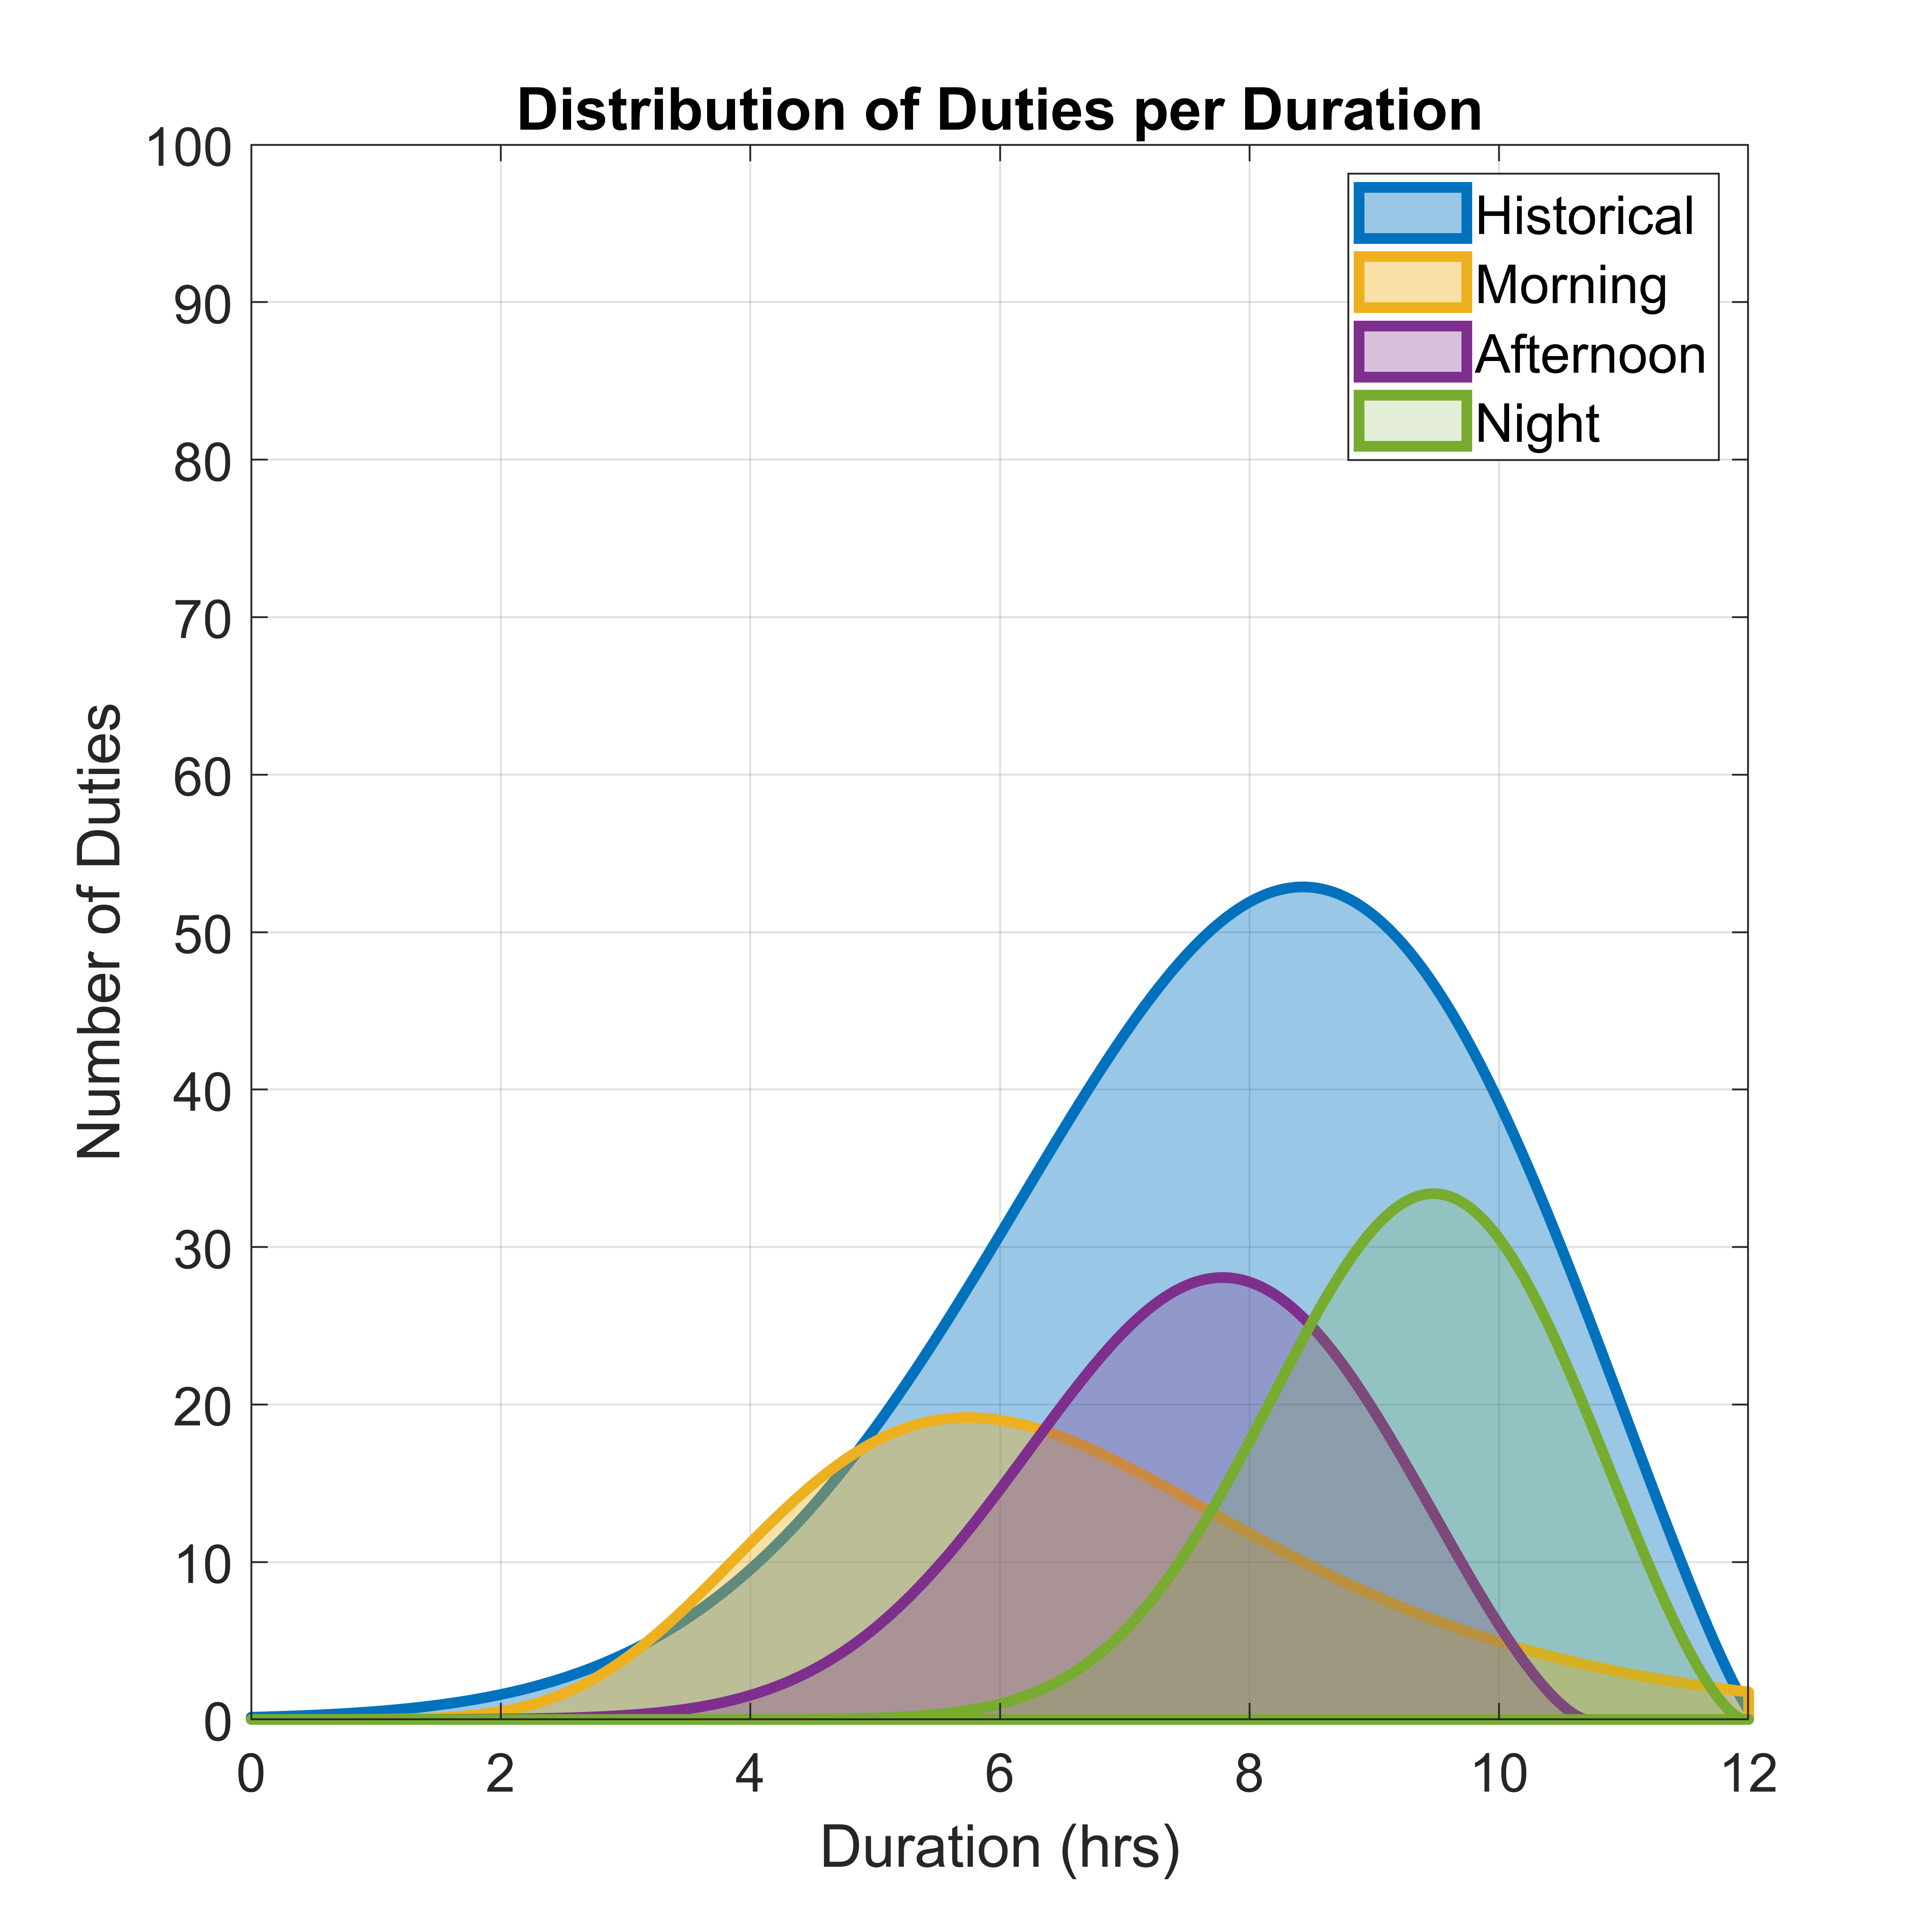
\includegraphics[width=0.46\linewidth]{[1] - chapter/Image Files/Waves-instances.png}
    
\end{center}
   \caption{The effect of splitting the Historical dataset into \textbf{wave instances} of the problem.}
\label{fig: Wave-instances.}
\end{figure}
\vspace*{4in}
